\documentclass[10pt]{article}
\usepackage[top=1.00in, bottom=1.0in, left=1.1in, right=1.1in]{geometry}
\renewcommand{\baselinestretch}{1.1}
\usepackage{graphicx}% http://ctan.org/pkg/graphicx
\usepackage{array}% http://ctan.org/pkg/array. Used to have images in table nicely 
\usepackage{natbib}
\usepackage{amsmath}
\usepackage{textcomp}
\usepackage[
singlelinecheck=false % <-- important
]{caption}
\usepackage{float}
\usepackage{hyperref}
\usepackage{xcolor}% change text colour 

\usepackage{atbegshi}% http://ctan.org/pkg/atbegshi
\AtBeginDocument{\AtBeginShipoutNext{\AtBeginShipoutDiscard}} % removes 1st empty page that would normally have a title on it 

\def\labelitemi{--}
\parindent=0pt


\graphicspath{ {./images/} }% tell latex where to find photos 

\begin{document}
\pagenumbering{gobble}%remove page numbers 
%\title{Winegrape Disease}
%\date{\today}
% \author{}
%\maketitle
\begin{table}[H]
\caption{A description of different diseases potentially afflicting winegrapes. This table comes from the Davis protocol. Photos: Lizzie, August 8, 2014.} % title of Table
%\centering % used for centering table. I dont want my tabel centred 
\begin{tabular}{ p{3cm}| l | p{4.5cm}| p{4.5cm}}  % left jusitfy columns ( l) or Wrap text after 4cm (p{4cm})
\hline\hline %inserts double horizontal lines
Problem & Photo example & Symptoms & Solution (always note issues in field data sheet!)\\ [0.5ex] % inserts table
%heading
\hline % inserts single horizontal line
Berry Rot 
	& % the and symbol seperates suff in each column 
	\raisebox{-\totalheight}{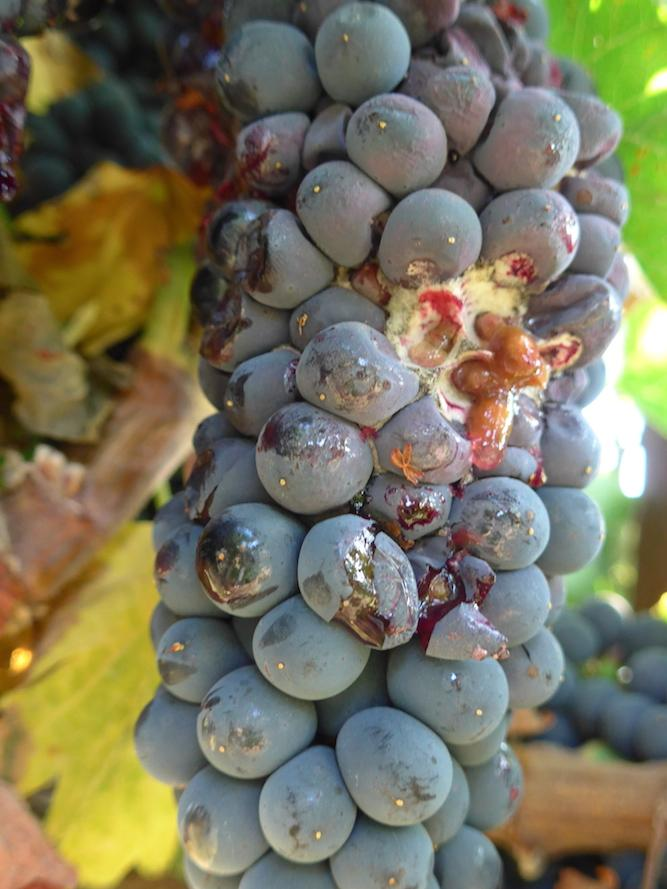
\includegraphics[scale=0.11]{BerryRot.jpg}} % scale sets the image size to be nice and small in this case. Raisebox makes the image in line with text.
	& Strong smell of fermentation; may see fungus; clusters looks ripe but berries basically dissolve into your hands upon touching (and now you’re happy to have gloves!)
	& Pick a different cluster to pull berries from! If all clusters on a vine are like this, do not sample (note on datasheet and take picture if possible)\\
\hline %inserts single line
Extreme berry shrivel: almost no berries left
	& \raisebox{-\totalheight}{\includegraphics[scale=0.11]{BerryShrivel2.jpg}} 
	& All clusters are missing berries or are very shriveled
	& Skip collecting berries from plant if all clusters look like this\\
\hline
Berry shrivel: a few berries left
	& \raisebox{-\totalheight}{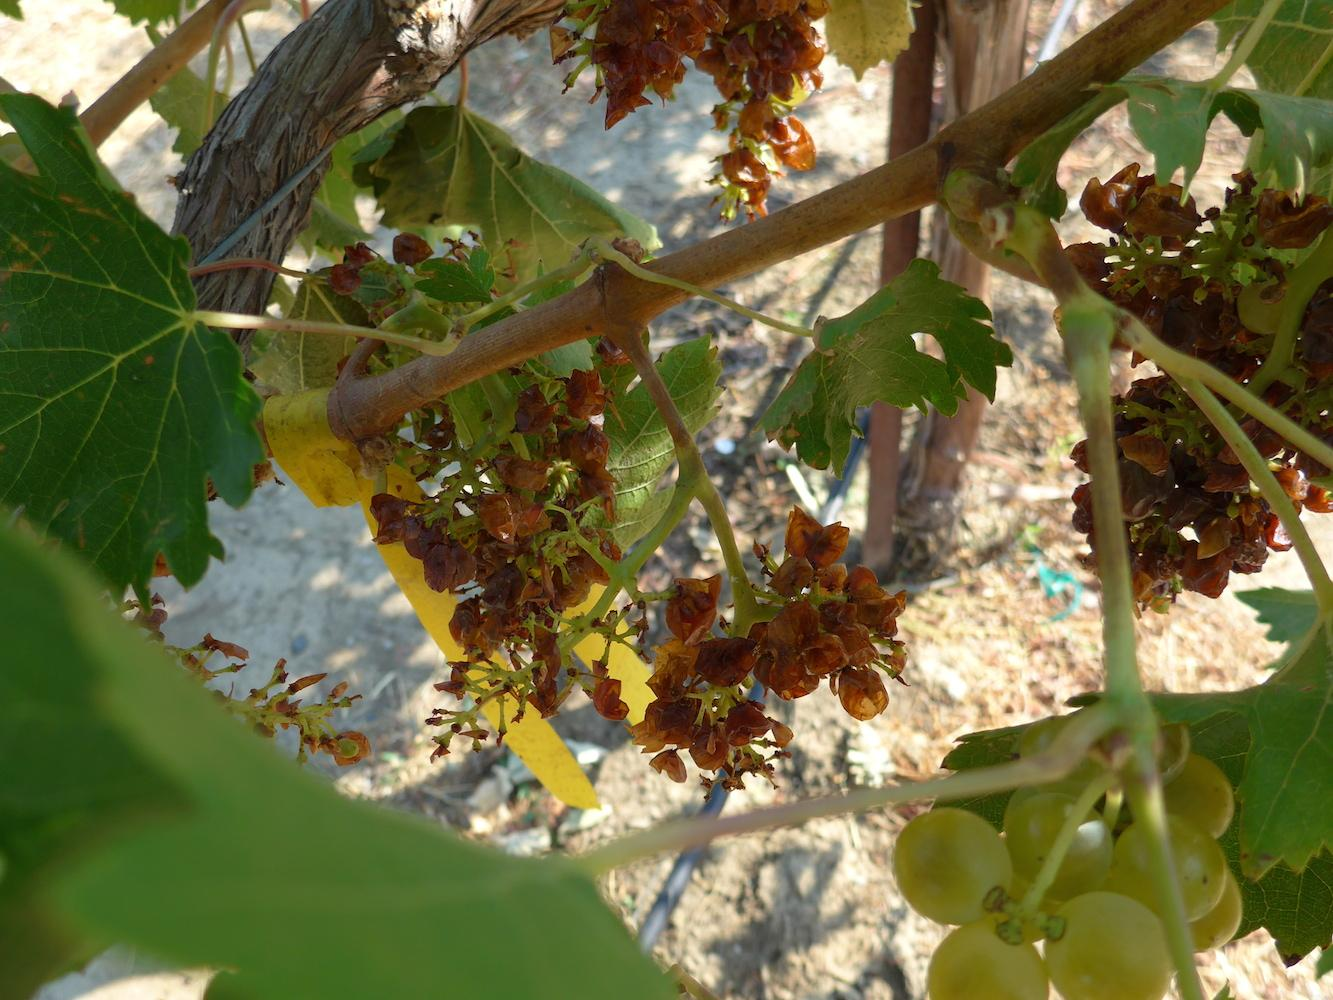
\includegraphics[scale=0.08]{BerryShrivel.jpg}} 
	& If certain clusters are fine, pick another clusters! If not, select five representative ‘good’ berries (do not pick any undeveloped berries)
	& Select five representative good berries if possible\\	
\hline
Chicken and hen
	& \raisebox{-\totalheight}{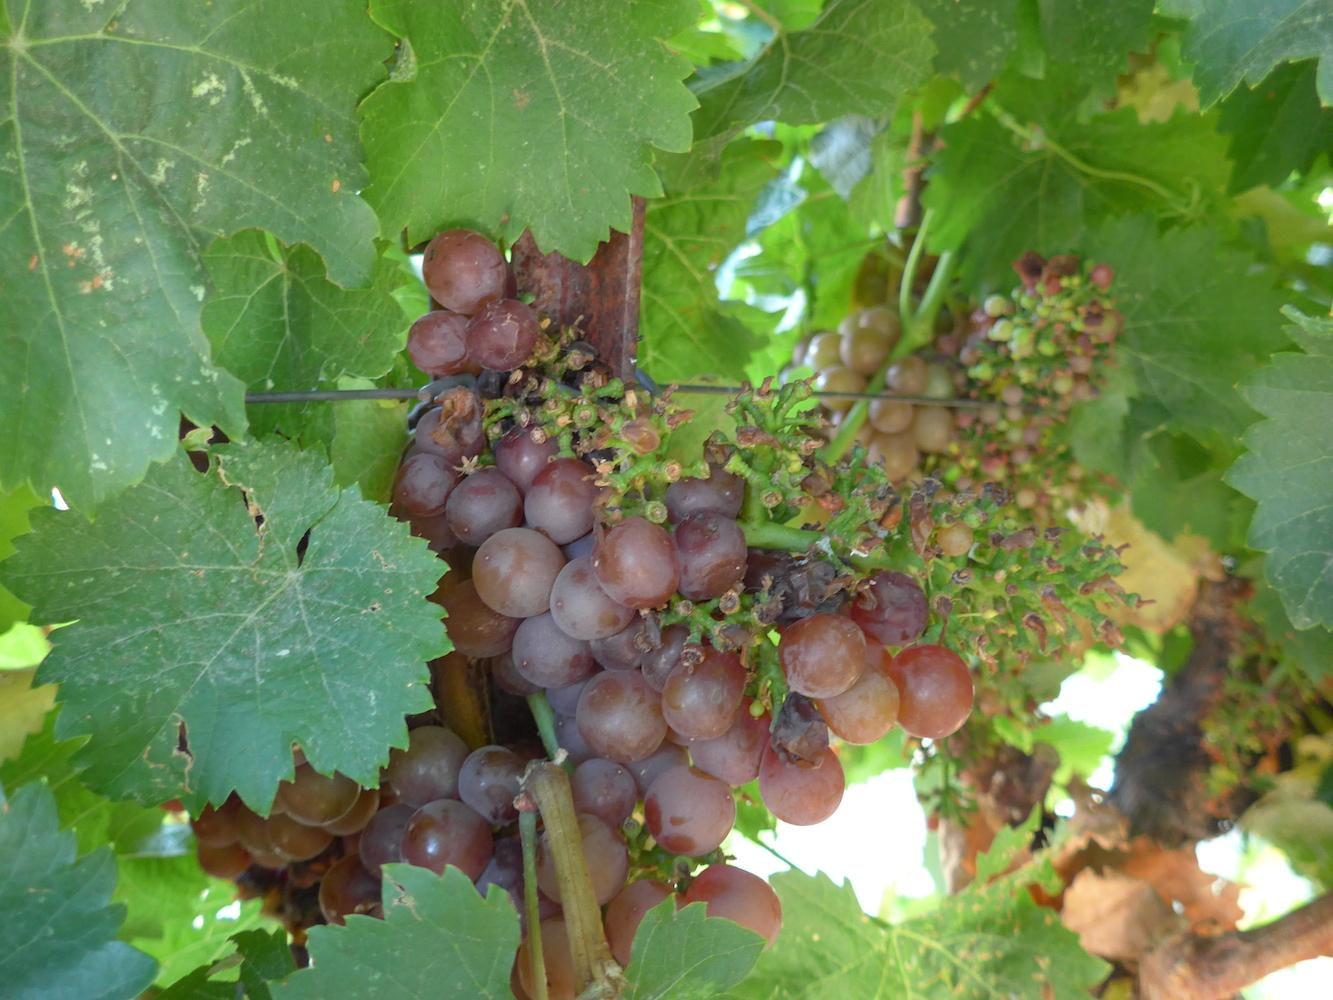
\includegraphics[scale=0.08]{Chicken.jpg}} 
	& Some of the cluster develops normally, some of the berries do not develop at all (shot berries) and some may appear to be missing 
	& If certain clusters are fine, pick another clusters! If not, select five representative ‘good’ berries (do not pick any undeveloped berries)\\
\hline
Not all berries done developing (but look like someday they will develop)
	& \raisebox{-\totalheight}{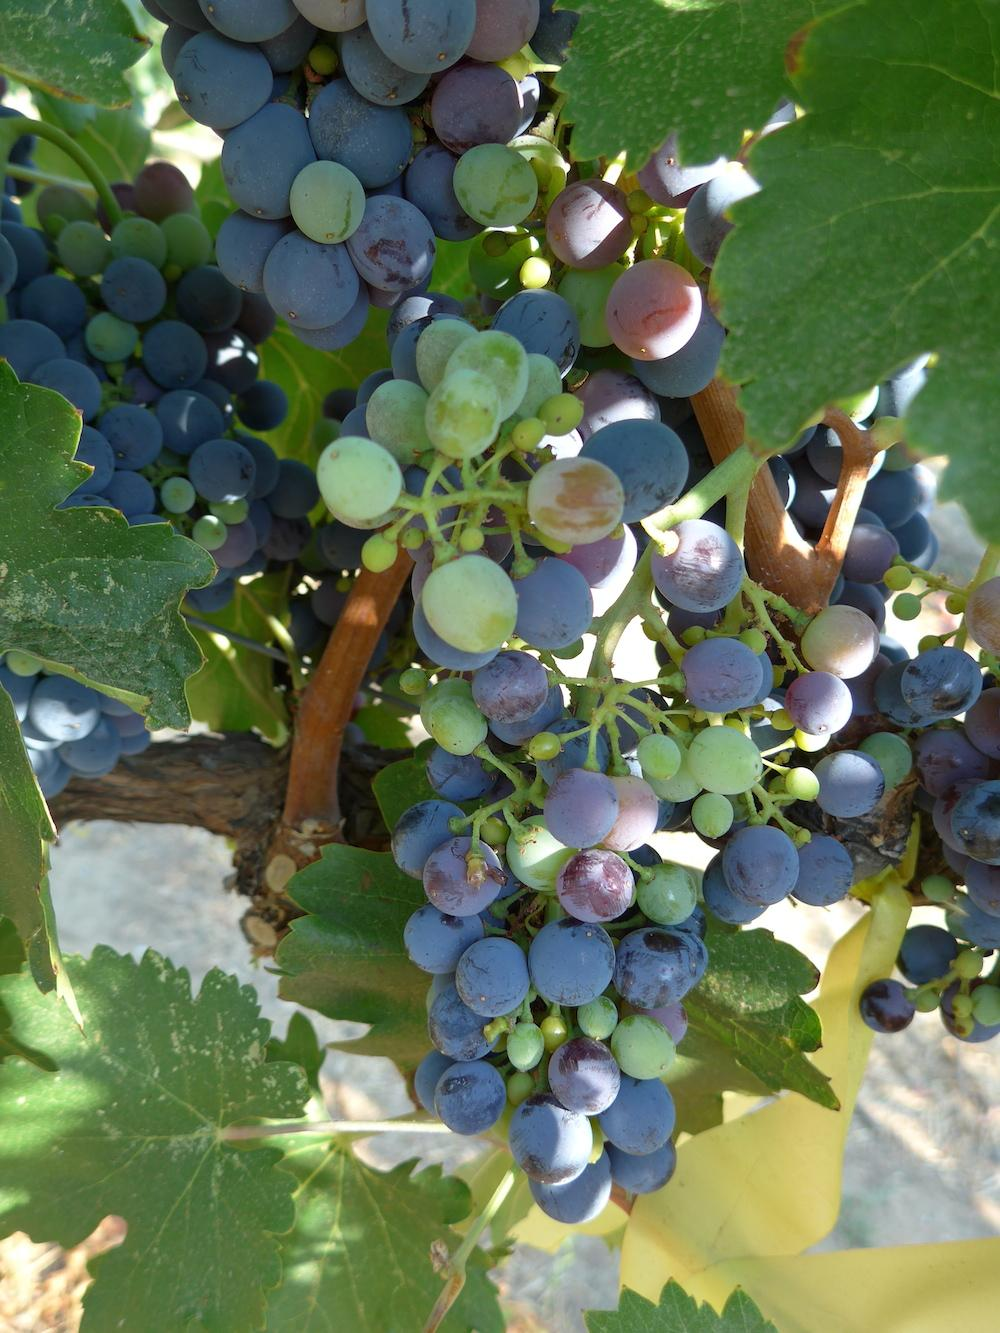
\includegraphics[scale=0.08]{Underdeveloped.jpg}} 
	& A few berries are undeveloped/green and rest are developed
	& Select a representative mix of berries; that is take 1 undeveloped berry if 20\% are undeveloped\\
\hline
Raisining
	& \textcolor{red}{\textbf{Need to add pic!}}
	& Berries are drying out as a result of over-ripening
	& Collect samples of raisined grapes, unless they are rock-hard and will be impossible to extract juice for measuring Brix. \textbf{For 2015 field season, consider a cutoff point after which resampling is not necessary (e.g., 30° Brix).} \\
\hline
\end{tabular}
\label{table:nonlin} % is used to refer this table in the text
\end{table}







\end{document}

This is a table of winegrape disease taken from the Davis protocol 